\chapter{Note-level description}
\label{chap:notelevel}
\begin{marginfigure}
\centering
\vspace{7cm}
\includesvg[pretex=\fontsize{6pt}{8pt}, width=1\linewidth]{images/applications/note.svg}
\vspace{0.1cm}
\caption{The hierarchy of notes is part of
the Note-level description of music, highlighted in red.}
\label{noteExtraction} 
\end{marginfigure}
The goal of this section is to illustrate how musical structures can be extracted for a constituent abstraction in our knowledge representation.
Musical structures can in general be divided in a frame-level, note-level, stream-level or notation-level description.
The note-level description of music often estimates the pitch, onset time and offset time in literature and corresponds to the descriptive constituents in the NOTE Hierarchy. We will first show why the estimation of those attributes requires the extraction of the fundamental frequencies, and will then extract them through a relative-harmonics based approach. This subset of fundamental frequencies will then be used in the hyperparameter-tuned DBSCAN clustering algorithm from Chapter \ref{chap:cluster} to recognize individual notes. Finally, we apply a power-based filter to enhance the extraction of notes from a resonance spectrum. This provides a refinement for the pitch extraction of notes. In the last section of this chapter, we also pitch our idea towards the extraction of harmonic overtones.

\section{Fundamental Frequency Detection}
\begin{marginfigure}
\centering
\vspace{3cm}
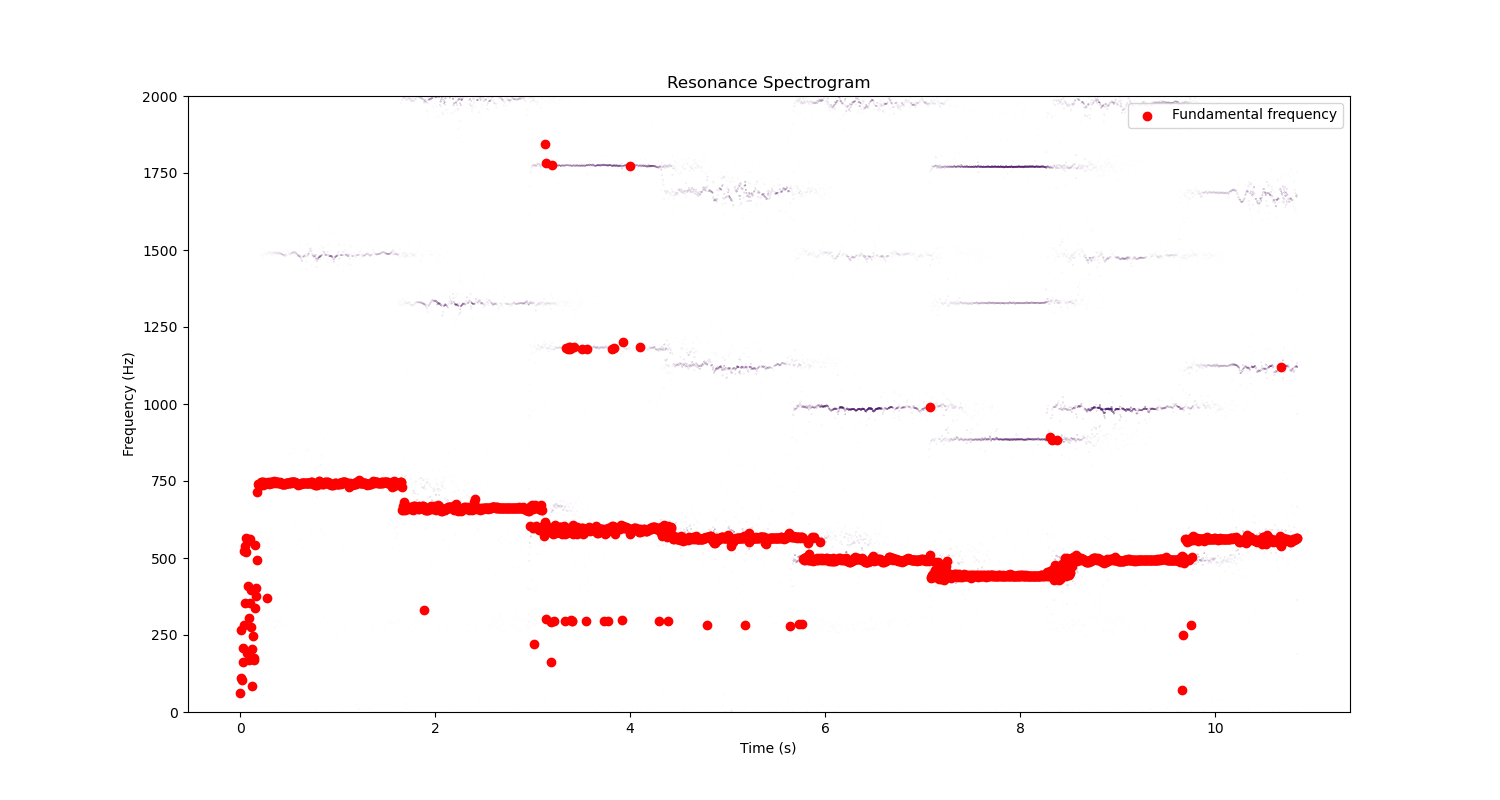
\includegraphics[width=1\linewidth]{images/cluster/violin_canonD_1_f0.png}
\caption{A slice (the first two measures) from a real audio recording of a violin performing \textit{Canon in D}, by Johann Pachelbel. Resonances that are estimated to belong to tonic root are highlighted in red.}
\label{rameauFundamental} 
\end{marginfigure}
As discussed earlier, musical instruments do not generate perfect sinusoidal waves. The reverberation of the sound in the environment, unique construction of the instrument, the inimitable single performance of a musician as well as the quality of recording equipment all contribute to the unique sound we capture in an audio recording. Noise, as well as harmonic and non-harmonic tones, interfere with each other, which makes the analysis of music relatively complex. 
Since humans perceive harmonics as a combination of overtones in harmonic series, we modelled the pitch perception by estimating the fundamental by the frequencies with the greatest relative harmonicity (Figure \ref{rameauFundamental}). Harmonicity refers to the distribution of power in a resonance, and since harmonic overtones are integer multiples of a fundamental tone, it is possible to estimate the fundamental, even in cases that the fundamental is missing, as was described in Chapter \ref{chap:Psychoacoustics} Psychoacoustics. For example, if a flute is playing an A4, the relative harmonicity with respect to A4 will be larger than the harmonicity of B4. The measurement of the relative harmonicity is examined through a resonance-harmonic inner product, described by \textcite{homer_modelling_2023} and defined as cosine similarity:

\begin{equation} 
S_C\left(f, H g_\eta-g_\eta\right)=\cos \theta=\frac{\operatorname{Re}\left[\left\langle f \mid H g_\eta-g_\eta\right\rangle\right]}{\|f\| \cdot\left\|H g_\eta-g_\eta\right\|}
\end{equation}

The fundamental frequency $\eta_0=\underset{\eta}{\arg \max }\left[S_C\left(f, H g_\eta-g_\eta\right)\right]$, which exactly estimates the frequencies with the greatest relative harmonicity.
\textcite{homer_modelling_2023} are also engaged in refining a method called the Rameau fundamental \sidenotemark\sidenotetext{Jean-Philippe \textcite{rameau_traite_1722} founded the modern musical theory with the publication \textit{Traité de l'harmonie réduite à ses principes naturels}, by mathematically proving that every pitch consists of a harmony. Rameau believed that the rules of harmony were derived from nature, called \textit{The vibrating world}, and these rules governed all music.}, which can currently be used for the Tonic root estimation, but should be further elaborated for recordings containing different instruments.


\section{Clustering}

\begin{marginfigure}
\centering
\vspace{1cm}
\includesvg[pretex=\fontsize{3pt}{5pt},width=1\linewidth]{images/cluster/e01pts4.svg}
\caption{$\epsilon$=0.1, minPts=4.}
\label{a} 
\end{marginfigure}


\begin{marginfigure}
\centering
\vspace{0.3cm}
\includesvg[pretex=\fontsize{3pt}{5pt},width=1\linewidth]{images/cluster/e01pts10.svg}
\caption{$\epsilon$=0.1, minPts=10.}
\label{b} 
\end{marginfigure}

\begin{marginfigure}
\centering
\vspace{0.3cm}
\includesvg[pretex=\fontsize{3pt}{5pt},width=1\linewidth]{images/cluster/e03pts4.svg}
\caption{$\epsilon$=0.3, minPts=10.}
\label{c} 
\end{marginfigure}





We performed the DBSCAN algorithm (discussed in Chapter \ref{chap:cluster}) on the detected fundamental frequencies in terms of frequency and onset to group resonances belonging to a certain note. In a slice (the first two measures) of a real audio recording of a violin performing \textit{Canon in D}, by Johann Pachelbel (\cite{bridget_stringspace_2019}), the DBSCAN algorithm has been performed with variable values of $\epsilon$ and $minPts$. Frequencies labeled with 0 are removed from the Figure \ref{clusteringRoot} and refer to all non-clustered resonances extracted from the audio file, frequencies labeled as -1 are labeled as noise from the Fundamental Frequency detection algorithm. 

\begin{figure}[h]
\centering
\includesvg[pretex=\fontsize{4pt}{6pt},width=0.9\linewidth]{images/applications/canonD.svg}
\vspace{0.1cm}
\caption{A correct labeling with the DBSCAN through correct parameter estimation. Performed on the first two measures of Canon in D.}
\label{clusteringRoot} 
\end{figure}

\subsection{Parameter estimation}

As mentioned earlier, $\epsilon$ and \textit{minPts} are the two parameters to be estimated. Variations in clustering when varying the two parameters are represented in Figures \ref{a}-\ref{c}. Therefore, we will introduce two automatic parameter estimators: the silhouette score and \textit{kneedle} method.


\subsubsection{Silhouette Score}
The silhouette score is a normalized metric for the evaluation of the quality of a clustering technique:

\begin{equation}
\text{silhouette score} = \frac{\beta-\alpha}{\max(\alpha,\beta)}.
\end{equation}

$\alpha$ denotes the average distance between the points inside a cluster, and $\beta$ the average distance between all clusters. A high positive value implies that the clusters are will distinct from one another, indicating a good clustering performance. Values close to 0 imply cluster overlapping, and negative scores tending towards -1 imply wrongly assigned points (\cite{rousseeuw_silhouettes_1987}).

\subsubsection{Kneedle Method}


Several methods exist to estimate an optimal value for $\epsilon$. Satopaa proposed the knee method in \textit{"Finding a "Kneedle" in a Haystack: Detecting Knee Points in System Behavior"} (\cite{satopaa_finding_2011}). From a k-distance graph, with values sorted from small to large (or vice versa), the optimal parameters can graphically be estimated by finding a knee or elbow in the graph as illustrated in Figure \ref{fig:kneedle}. 
The mathematical definition of the curvature is the basis definition for the knee estimate. \textcite{satopaa_finding_2011} defined the Kneedle-algorithm as following:

\begin{marginfigure}
\vspace{2cm}
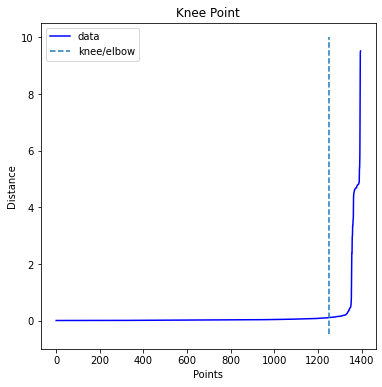
\includegraphics[width=1\linewidth]{images/cluster/kneePoint.png}
\caption{Kneedle of a harmonic series from C5 to F played by a flute.}
\label{fig:kneedle} 
\end{marginfigure}

\begin{definition}[Kneedle]
For a continuous function $f$, there exists a $K_f(x)$ that defines the curvature of $f$ at any point as a function of its first and second derivative:
\begin{equation}
K_f(x)=\frac{f^{\prime \prime}(x)}{\left(1+f^{\prime}(x)^2\right)^{1.5}}.
\end{equation}
\end{definition}

The point of maximum curvature is used in the Kneedle-algorithm to select the optimal value for $\epsilon$, which is (1 - normalized value) of the knee locator (or just the normalized value if inverse density ordering was implemented). It is worth mentioning that the clustering results are significantly impacted by the choice of $\epsilon$. A small value of $\epsilon$ will lead to inadequate clustering, whereas a high value will result in most objects being merged into a single cluster.


\subsection{Clustering Performance Evaluation}

The rule of thumb for a threshold value of the minimum amount of neighbors within a radius $\epsilon$, is \textit{minPts} = dim$*2$ (\cite{ester_density-based_1996, sander_density-based_1998}). However, if the dataset is large or contains noisy data, a larger value for \textit{minPts} can be required. The threshold value was therefore estimated with the silhouette score and a method comparison study for the $\epsilon$-estimation was performed to evaluate the difference between the Kneedle-algorithm and silhouette score on the quality of clustering. We examined the detection of 159 synthetically generated notes. The evaluated notes differ in duration, pitch and distance. The hit or miss criterion was based on whether a group of resonances representing a note was detected or not. We noticed that the silhouette score performed a significantly better clustering than the \textit{kneedle} method. However, in both methods, due to the not-yet-perfect $f_0$ estimation, noise was clustered together and influences the results. 

\subsection{Clusters of noise} 
In this specific section, when we mention \textit{noise}, we are referring to resonances that are detected along with the fundamental tone, even though they are not actually part of it. Most of them are classified as -1 by the DBSCAN algorithm, but closely laying noisy points form sometimes unwanted little clusters of overtones. However, they mostly have a relatively low power compared to the resonances presented in the real fundamental. 
Therefore, we removed the clusters containing a significantly lower power on average. The difference between a plot with and without power is shown in Figure \ref{remove_lowpower}. It is crucial to get rid of these clusters of noise for attributing constituents to a particular note in our system, as well as for the musical transcription of the sound.

\begin{figure}[h]
\centering
\includesvg[pretex=\fontsize{4pt}{6pt},width=1\linewidth]{images/cluster/remove_lowpower.svg}
\caption{A comparison between two three-dimensional plots with a third axis denoting the power. Clusters with a small average power, relative to the other ones, are removed.}
\label{remove_lowpower} 
\end{figure}



\section{Attributing a Note Constituent}
Resonances belonging to a cluster are each assigned to a constituent representing a musical \textit{note}, attributed with the average frequency, onset, off-set and relative duration. Extracting the real rhythm of a live performance is more complicated than it seems, since people never play perfectly on the beat as written on paper. Therefore, we focused on the accurate extraction of pitch for this thesis, and suggested a relative estimation of the duration in our software. It correctly estimates the duration of notes for computer-generated audio files, but needs a refinement for audio files performed by humans in future work. 


\subsubsection{Example: Syrinx (Flute Solo)}
\begin{figure}[h]
\centering
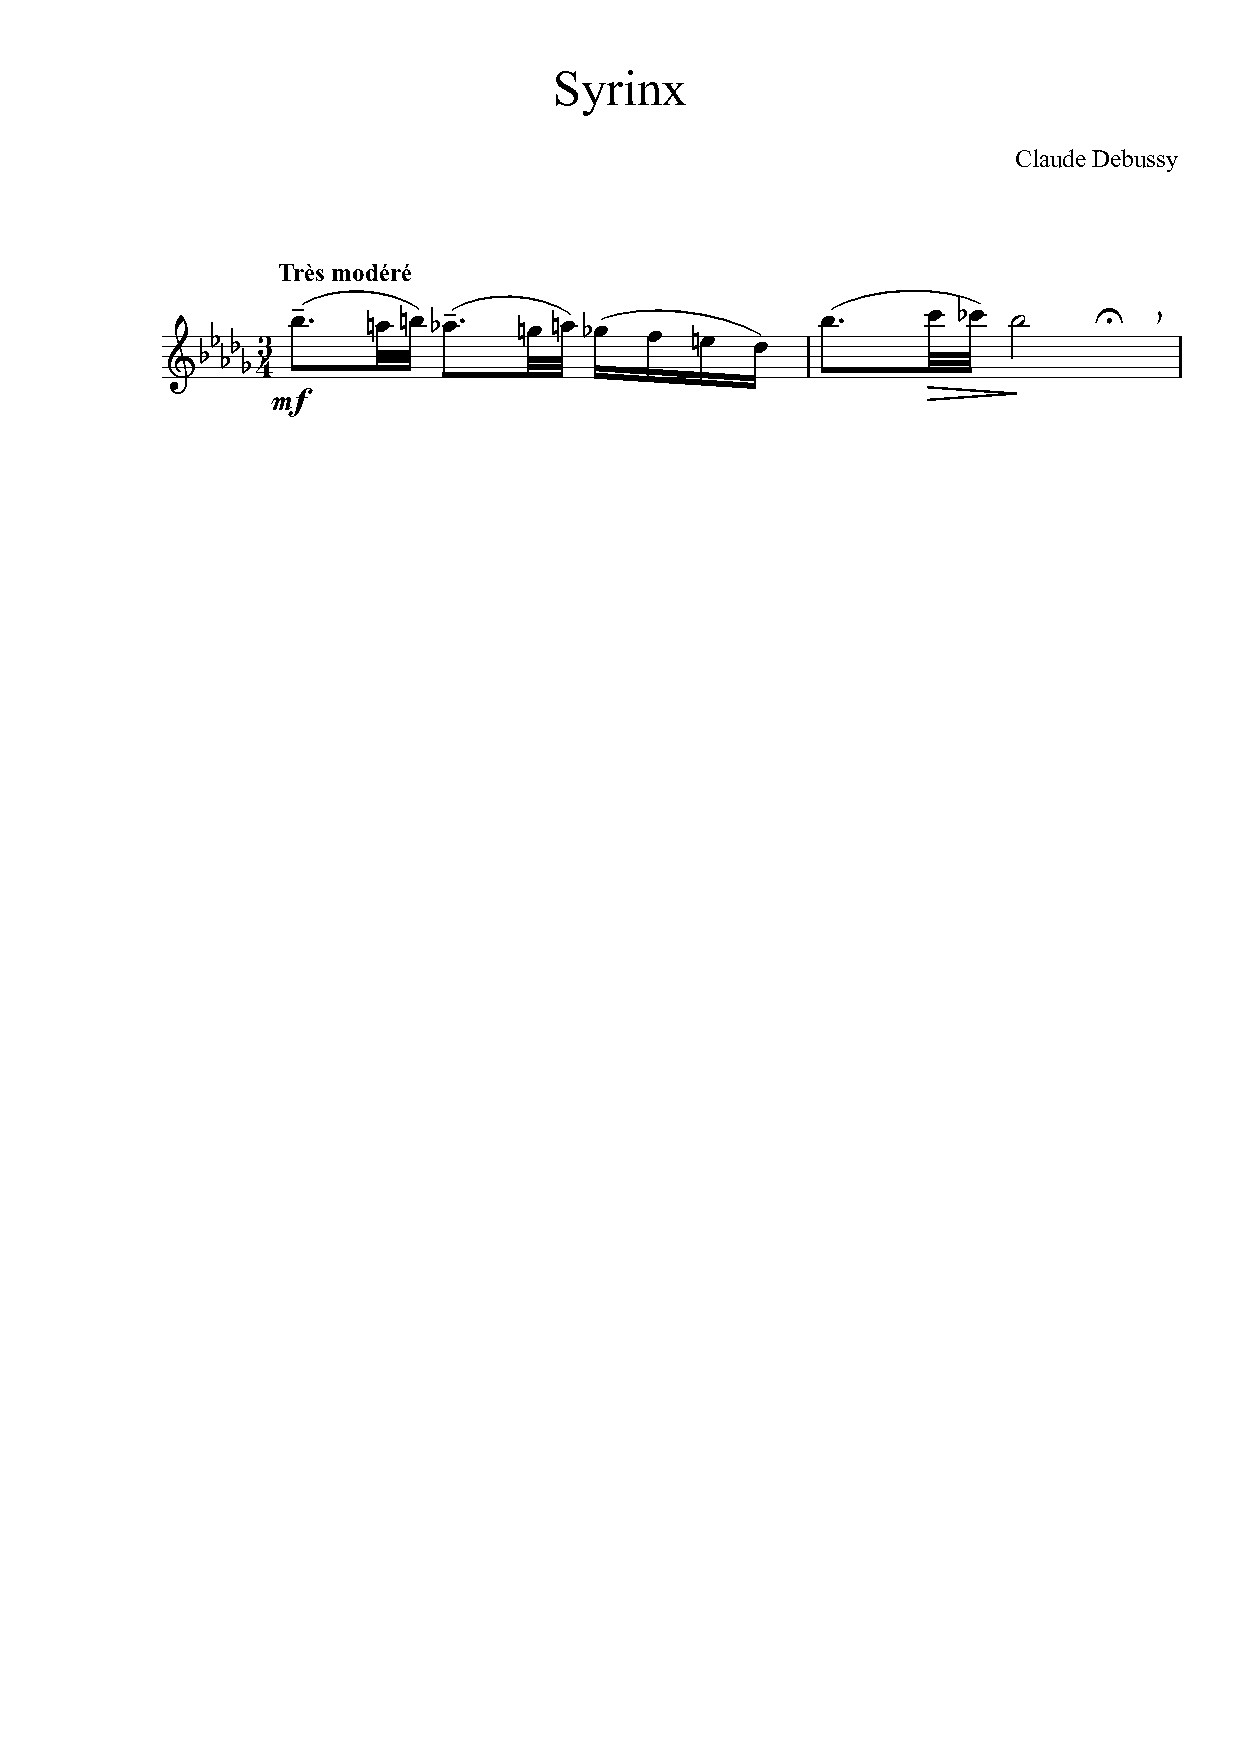
\includegraphics[width=1\linewidth]{images/applications/syrinx_original.pdf}
\caption{Western score notation of the first two measures of Syrinx, by Claude Debussy.}
\label{syrinx_original} 
\end{figure}
We analyzed the pitch estimation of a slice of \textit{Syrinx}, by Claude Debussy, performed by a real and artificially generated flute. The ground truth music score is presented in Figure \ref{syrinx_original}.
The first two measures have strong variations in rhythm and the notes are laying nearby, which makes is harder for the cluster algorithm to recognize two different objects. With the application of our method on this sample, the pitch of each note was correctly reconstructed based on the frequency data within each cluster. Please note that there is a slight difference in notation due to the key signature in the original piece. Thus, the pitch of each note in this slice has been assigned correctly\sidenotemark\sidenotetext{About musical notation: The flat ($\flat$), sharp ($\sharp$), and natural ($\natural$) signs preceding a note indicate that the note should be played a semitone lower, higher, or disregarding the sign in the key signature or the modification of a tone within the same measure.}, as illustrated in Figure \ref{syrinx_artificial}.


\begin{figure}[h]
\centering
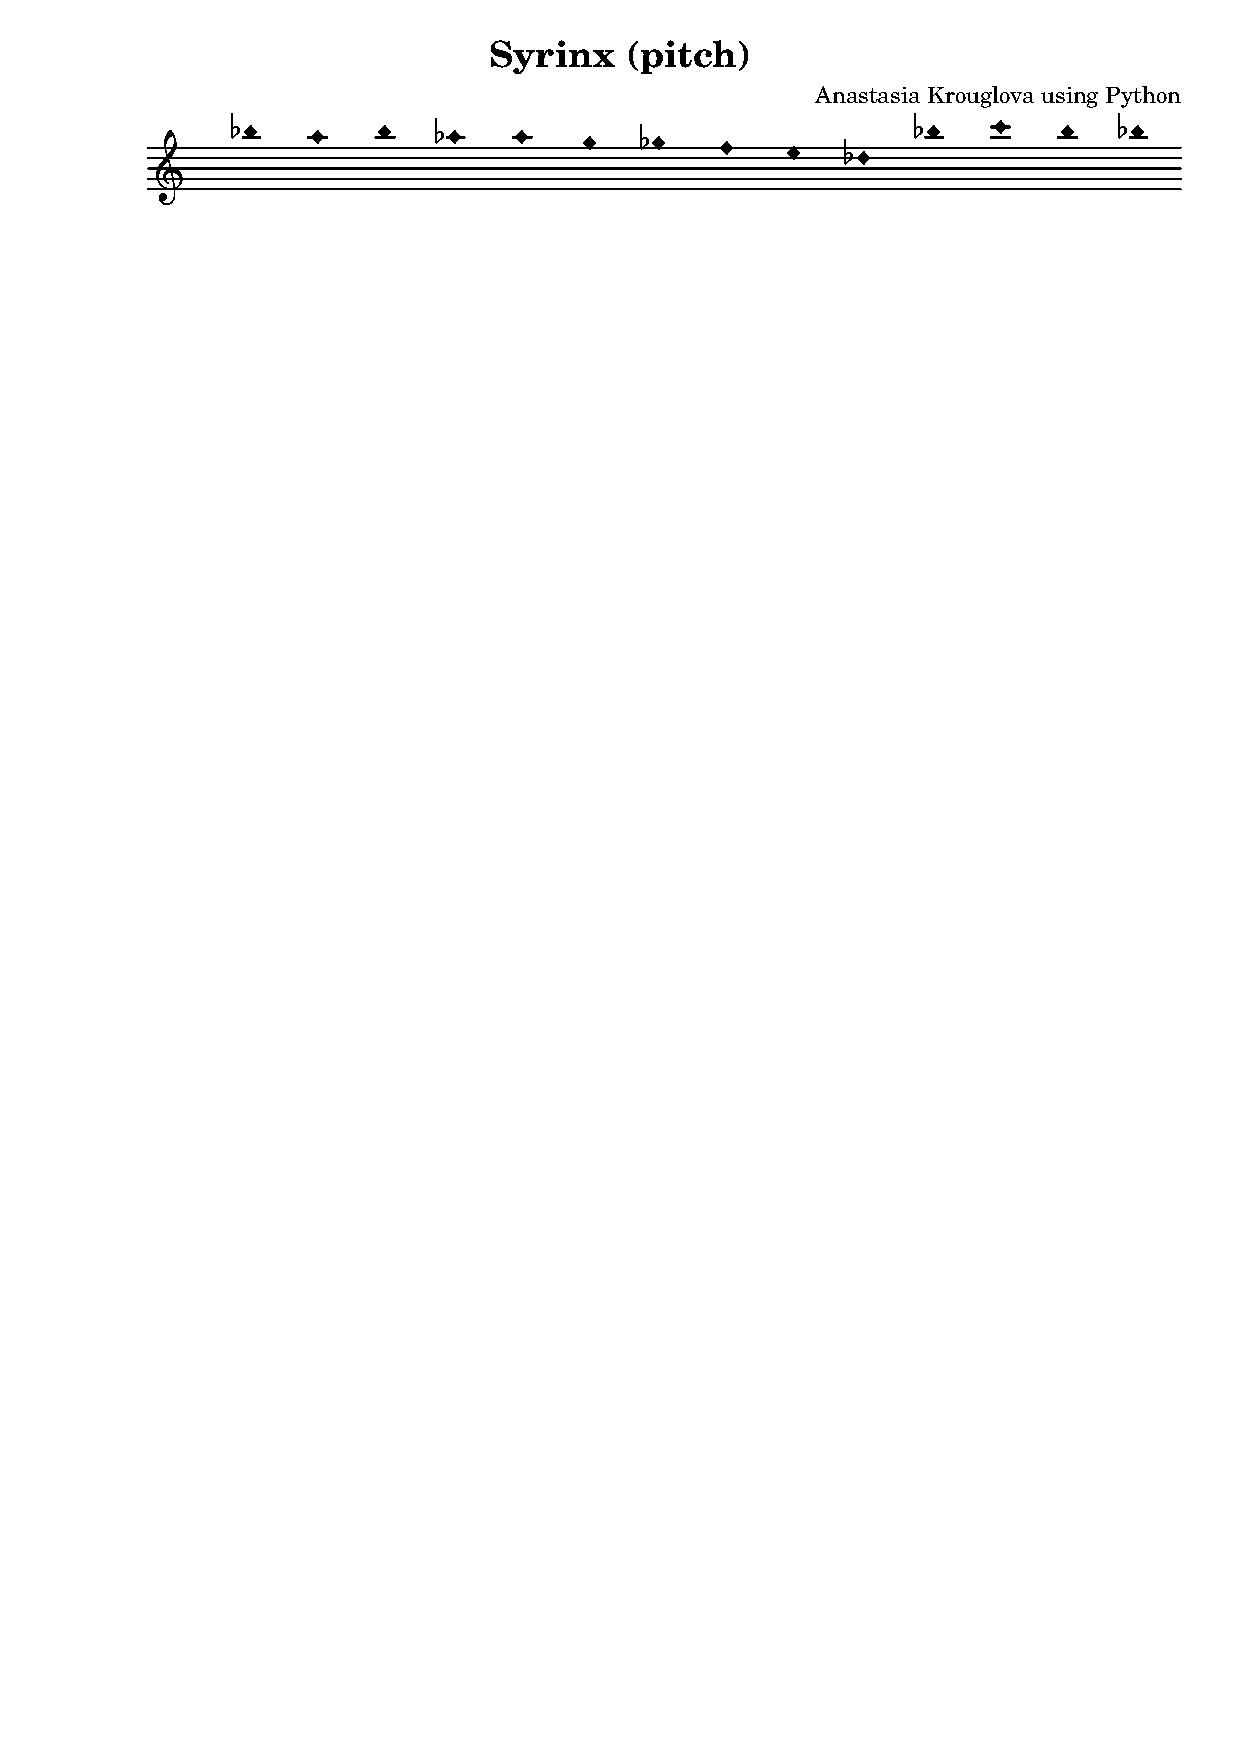
\includegraphics[width=0.9\linewidth]{images/applications/pitches_syrinx.pdf}
\caption{The pitches in the first measure of Syrinx, by Claude Debussy were correctly assigned and serve as one of the attributes for the Note constituent.}
\label{syrinx_artificial} 
\end{figure}

\begin{marginfigure}
\centering
\vspace{1.8cm}
\includesvg[pretex=\fontsize{6pt}{8pt}, width=1\linewidth]{images/applications/harm.svg}
\vspace{0.1cm}
\caption{The hierarchy of harmonics is part of the Frame-level description of music, highlighted in purple.}
\label{harmonyExtraction} 
\end{marginfigure}


\section{Towards a Frame-level description}
We introduce our approach towards a subtask of the frame-level description of music, namely the extractions of harmonic overtones. The frame-level description (i.e., multi-pitch estimation) estimates the number of notes that are simultaneously played in a slice of time (\cite{benetos_automatic_2019}). It is currently based on the assumption that the fundamental tone is known, but should be expanded to a relative estimation and extraction of overtones for polyphonic music.


\subsection{Attributing the Harmonic Constituent}
As discussed in the chapter about psychoacoustics, a real musical tone often consists of a fundamental, but also from harmonic and non-harmonic overtones. Since harmonic overtones are integer multiples of the fundamental tones, they can be found by defining them in a space of the so-called $f_0$-likeliness ($H$):

\begin{equation}
    H = E(\frac{f}{f_0} \mod{1})
\end{equation}

\begin{marginfigure}
\centering
\includesvg[pretex=\fontsize{3.3pt}{5pt}, width=1.12\linewidth]{images/cluster/canonD_overtones.svg}
\vspace{0.1cm}
\caption{The extraction of the harmonic overtone from a real audio recording performed by \textcite{bridget_stringspace_2019} (produced and approved for use by Stringspace).}
\label{overtonesPlot} 
\end{marginfigure}



$E \sim \mathcal{N}(0.5, 0.5)$ simulates the idea of entropy for the definition of how likely a resonance is part of an overtone.
We used a real audio recording of a violin performing Canon in D, by Johann Pachelbel (\cite{bridget_stringspace_2019}) to analyze the overtones of a violin. We limited the space with a bound defined in the $H$ space, which give us a first approximation of the overtones if the fundamental is known.